% !TeX program = xelatex
\documentclass[notheorems]{beamer}

\mode<presentation>
{
  \usetheme{Antibes}
  \setbeamertemplate{footline}[frame number]{}
  \setbeamertemplate{navigation symbols}{}
}

\usepackage{amsmath}
\usepackage{xeCJK}
\setCJKsansfont[ItalicFont={Microsoft YaHei}]{Microsoft YaHei}

\usepackage{ragged2e}
\justifying\let\raggedright\justifying

\makeatletter
\newenvironment<>{proofs}[1][\proofname]{
    \par
    \def\insertproofname{#1\@addpunct{.}}
    \usebeamertemplate{proof begin}#2}
  {\usebeamertemplate{proof end}}

  \newenvironment<>{solution}[1][Solution.]{
    \par
    \def\insertproofname{#1\@addpunct{.}}
    \usebeamertemplate{proof begin}#2}
  {\usebeamertemplate{proof end}}

  \newtheorem*{definition}{Definition}
  \newtheorem{example}{Example}[section]
  \newtheorem{theorem}{Theorem}[section]
  \newtheorem{property}{Property}[section]
\makeatother

\setbeamertemplate{theorems}[numbered]

\setbeamertemplate{section in toc}[sections numbered]
\setbeamertemplate{subsection in toc}[subsections numbered]

\numberwithin{equation}{section}
\numberwithin{equation}{subsection}

\usefonttheme[onlymath]{serif}
\providecommand{\Arg}{\operatorname{Arg}}
\providecommand{\Ln}{\operatorname{Ln}}
\providecommand{\Arcsin}{\operatorname{Arcsin}}
\providecommand{\Arccos}{\operatorname{Arccos}}
\providecommand{\Arctan}{\operatorname{Arctan}}
\providecommand{\Arcsinh}{\operatorname{Arcsinh}}
\providecommand{\Arccosh}{\operatorname{Arccosh}}
\providecommand{\Arctanh}{\operatorname{Arctanh}}
\providecommand{\abs}[1]{\left\lvert#1\right\rvert}

\title{Chapter 2: Analytic Functions}
\author{Taotao Wang, Associate Professor}
\institute{College of Electronics and Information Engineering, Shenzhen University}

\begin{document}

\everymath{\displaystyle}

\begin{frame}
	\titlepage
\end{frame}

\begin{frame}{Outline}
	\tableofcontents
\end{frame}

\section{Concept of Analytic Functions}

\begin{frame}
	\frametitle{Outline}
	\tableofcontents[currentsection]
\end{frame}

\begin{frame}
	\begin{enumerate}
		\item \textbf{Derivatives of Complex Functions}
		      \begin{enumerate}[1)]
			      \item Definition of the Derivative
			            \begin{definition}
				            Let $w=f(z)$ be defined in a domain $D$, and let $z_0\in D$ and $z_0+\Delta z\in D$. If the limit
				            \[\lim_{\Delta z\to 0}\frac{f(z_0+\Delta z)-f(z_0)}{\Delta z}\]
				            exists (and is finite), then $f(z)$ is said to be differentiable（可导） at $z_0$.
			            \end{definition}
		      \end{enumerate}
	\end{enumerate}
\end{frame}

\begin{frame}
	\begin{enumerate}
		\setcounter{enumi}{1}
		\item []
		      \begin{enumerate}[1)]
			      \item []
			            \begin{definition}[Cont.]
				            This limit is called the derivative（导数） of $f(z)$ at $z_0$ and is denoted by
				            \[f'(z_0)=\left.\frac{\mathrm{d}w}{\mathrm{d}z}\right|_{z=z_0}=\lim_{\Delta z\to 0}\frac{f(z_0+\Delta z)-f(z_0)}{\Delta z}. \tag{2.1.1}\]
				            Equivalently, for every $\varepsilon>0$ there is a $\delta(\varepsilon)>0$ such that $0<\abs{\Delta z}<\delta$ implies
				            \[\abs{\frac{f(z_0+\Delta z)-f(z_0)}{\Delta z}-f'(z_0)}<\varepsilon.\]
				            As for limits in Chapter 1, $\Delta z\to0$ may happen along any path.
			            \end{definition}
		      \end{enumerate}
	\end{enumerate}
\end{frame}

\begin{frame}
	\begin{example}
		Determine whether the following functions are differentiable:
		\begin{enumerate}
			\item $f(z)=z^2$;
			\item $f(z)=2x+yi$.
		\end{enumerate}
	\end{example}
	\begin{solution}<2->
		\begin{enumerate}
			\item For every $z$ in the complex plane,
			      \begin{align*}
				      \lim_{\Delta z\to 0}\frac{f(z+\Delta z)-f(z)}{\Delta z} & =\lim_{\Delta z\to 0}\frac{(z+\Delta z)^2-z^2}{\Delta z} \\
				                                                              & =\lim_{\Delta z\to 0}(2z+\Delta z)=2z.
			      \end{align*}
			      Hence $f(z)=z^2$ is differentiable everywhere, and $f'(z)=2z$.
		\end{enumerate}
	\end{solution}
\end{frame}

\begin{frame}
	\begin{solution}[Solution\ (Cont.)]
		\begin{enumerate}
			\setcounter{enumi}{1}
			\item With $\Delta z=\Delta x+i\Delta y$,
			      \begin{align*}
				      \frac{f(z+\Delta z)-f(z)}{\Delta z} & =\frac{2(x+\Delta x)+(y+\Delta y)i-(2x+yi)}{\Delta x+i\Delta y} \\
				                                          & =\frac{2\Delta x+i\Delta y}{\Delta x+i\Delta y}.
			      \end{align*}
			      If $z+\Delta z\to z$ along a line parallel to the real axis (Figure 2.1), then $\Delta y=0$ and the quotient equals $\frac{2\Delta x}{\Delta x}=2$.

			      If $z+\Delta z\to z$ along a line parallel to the imaginary axis, then $\Delta x=0$ and the quotient equals $\frac{i\Delta y}{i\Delta y}=1$.

			      The two limits differ, so $f(z)=2x+yi$ is differentiable nowhere.
		\end{enumerate}
	\end{solution}
\end{frame}

\begin{frame}
	\begin{solution}[Solution\ (Cont.)]
		\begin{figure}
			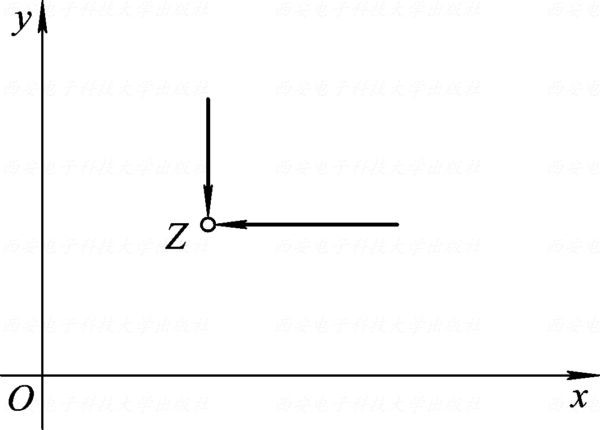
\includegraphics[height=0.6\textheight]{Figure_2_1.jpg}
			\caption{2.1}
		\end{figure}
	\end{solution}
\end{frame}

\begin{frame}
	\begin{enumerate}
		\setcounter{enumi}{1}
		\item []
		      \begin{enumerate}[1)]
			      \setcounter{enumii}{1}
			      \item Differentiability and Continuity\\
			            Suppose $f(z)$ is differentiable at $z_0$. Let
			            \[\rho(\Delta z)=\frac{f(z_0+\Delta z)-f(z_0)}{\Delta z}-f'(z_0). \tag{2.1.2}\]
			            By the definition of the derivative,
			            \[\lim_{\Delta z\to 0}\rho(\Delta z)=0.\]
		      \end{enumerate}
	\end{enumerate}
\end{frame}

\begin{frame}
	\begin{enumerate}
		\setcounter{enumi}{1}
		\item []
		      \begin{enumerate}[1)]
			      \setcounter{enumii}{1}
			      \item []
			            From (2.1.2),
			            \[f(z_0+\Delta z)=f(z_0)+f'(z_0)\Delta z+\rho(\Delta z)\Delta z, \tag{2.1.3}\]
			            and therefore
			            \[\lim_{\Delta z\to 0}f(z_0+\Delta z)=f(z_0).\]
			            Thus, differentiability at $z_0$ implies continuity at $z_0$.

			            The converse is false: $f(z)=2x+yi$ is continuous everywhere but differentiable nowhere.
		      \end{enumerate}
	\end{enumerate}
\end{frame}

\begin{frame}
	\begin{enumerate}
		\setcounter{enumi}{1}
		\item []
		      \begin{enumerate}[1)]
			      \setcounter{enumii}{2}
			      \item Rules of Differentiation\\
			            Complex derivatives obey the same rules as real derivatives:
			            \begin{enumerate}[a)]
				            \item $(c)'=0$, where $c$ is a complex constant;
				            \item $(z^n)'=nz^{n-1}$, where $n$ is a positive integer;
				            \item $[f(z)\pm g(z)]'=f'(z)\pm g'(z)$;
				            \item $[f(z)g(z)]'=f'(z)g(z)+f(z)g'(z)$;
				            \item $\left[\frac{f(z)}{g(z)}\right]'=\frac{f'(z)g(z)-f(z)g'(z)}{g^2(z)}$, where $g(z)\neq 0$;
				            \item $\{f[g(z)]\}'=f'(w)g'(z)$, where $w=g(z)$ (chain rule);
				            \item $f'(z)=\frac{1}{\varphi'(w)}$, where $w=f(z)$ and $z=\varphi(w)$ are mutually inverse single-valued functions and $\varphi'(w)\neq 0$.
			            \end{enumerate}
		      \end{enumerate}
	\end{enumerate}
\end{frame}

\begin{frame}
	\begin{enumerate}
		\setcounter{enumi}{1}
		\item []
		      \begin{enumerate}[1)]
			      \setcounter{enumii}{3}
			      \item Differential\\
			            As in real analysis, suppose $w=f(z)$ is differentiable at $z_0$. By (2.1.3),
			            \[\Delta w=f(z_0+\Delta z)-f(z_0)=f'(z_0)\Delta z+\rho(\Delta z)\Delta z,\]
			            where $\lim_{\Delta z\to 0}\rho(\Delta z)=0$.
			            Hence $\rho(\Delta z)\Delta z$ is an infinitesimal of higher order than $\Delta z$, and $f'(z_0)\Delta z$ is the linear principal part of $\Delta w$.
		      \end{enumerate}
	\end{enumerate}
\end{frame}

\begin{frame}
	\begin{enumerate}
		\setcounter{enumi}{1}
		\item []
		      \begin{enumerate}[1)]
			      \setcounter{enumii}{3}
			      \item []
			            The linear part $f'(z_0)\Delta z$ is called the differential（微分） of $w=f(z)$ at $z_0$:
			            \[\mathrm{d}w=f'(z_0)\Delta z. \tag{2.1.4}\]
			            For $f(z)=z$ we have $\mathrm{d}z=\Delta z$, so (2.1.4) becomes $\mathrm{d}w=f'(z_0)\,\mathrm{d}z$, that is,
			            \[f'(z_0)=\left.\frac{\mathrm{d}w}{\mathrm{d}z}\right|_{z=z_0}. \tag{2.1.5}\]
			            Thus, a function has a differential at $z_0$ if and only if it has a derivative at $z_0$. If $f(z)$ is differentiable at every point of a domain $D$, it is said to be differentiable in $D$.
		      \end{enumerate}
	\end{enumerate}
\end{frame}

\begin{frame}
	\begin{enumerate}
		\setcounter{enumi}{1}
		\item \textbf{Analytic Functions}
		      \begin{definition}
			      If $f(z)$ is differentiable at $z_0$ and at every point of some neighborhood of $z_0$, then $f(z)$ is said to be analytic（解析） at $z_0$. If $f(z)$ is analytic at every point of a domain $D$, then $f(z)$ is said to be analytic in $D$, or an analytic function in $D$.

			      If $f(z)$ is not analytic at $z_0$, then $z_0$ is called a singular point（奇点） of $f(z)$.
		      \end{definition}
		      \begin{enumerate}
			      \item []
			            Analyticity is a neighborhood property: differentiability at a single point is not enough.
		      \end{enumerate}
	\end{enumerate}
\end{frame}

\begin{frame}
	\begin{example}
		Investigate the analyticity of the following functions:
		\begin{enumerate}
			\item $f(z)=z^2$;
			\item $f(z)=2x+yi$;
			\item $f(z)=\abs{z}^2$;
			\item $f(z)=1/z$.
		\end{enumerate}
	\end{example}
	\begin{solution}<2->
		\begin{enumerate}
			\item[(1)(2)] By Example 1.1, $f(z)=z^2$ is analytic in the whole plane, while $f(z)=2x+yi$ is analytic nowhere.
			\item[(4)] $f(z)=1/z$ is differentiable for $z\neq0$ with $f'(z)=-1/z^2$, so it is analytic in $\mathbb{C}\setminus\{0\}$, and $z=0$ is a singular point.
		\end{enumerate}
	\end{solution}
\end{frame}

\begin{frame}
	\begin{solution}[Solution\ (Cont.)]
		\begin{enumerate}
			\item[(3)] For $f(z)=\abs{z}^2=z\overline z$,
			      \begin{align*}
				      \frac{f(z_0+\Delta z)-f(z_0)}{\Delta z} & =\frac{(z_0+\Delta z)(\overline{z_0}+\overline{\Delta z})-z_0\overline{z_0}}{\Delta z} \\
				                                               & =\overline{z_0}+\overline{\Delta z}+z_0\frac{\overline{\Delta z}}{\Delta z}.
			      \end{align*}
			      If $z_0=0$, the quotient equals $\overline{\Delta z}\to0$, so $f'(0)=0$.
		\end{enumerate}
	\end{solution}
\end{frame}

\begin{frame}
	\begin{solution}[Solution\ (Cont.)]
		\begin{enumerate}
			\item[] If $z_0\neq 0$, let $z_0+\Delta z\to z_0$ along the line $y-y_0=k(x-x_0)$. Then
			\[\frac{\overline{\Delta z}}{\Delta z}=\frac{\Delta x-i\Delta y}{\Delta x+i\Delta y}=\frac{1-ik}{1+ik},\]
			which depends on $k$, so the limit does not exist.

			Therefore, $f(z)=\abs{z}^2$ is differentiable only at $z=0$ and is analytic nowhere.
		\end{enumerate}
	\end{solution}
\end{frame}

\begin{frame}
	\begin{theorem}
		\begin{enumerate}
			\item If $f(z)$ and $g(z)$ are analytic in a domain $D$, then $f\pm g$, $fg$, and $f/g$ (where $g(z)\neq0$) are analytic in $D$.
			\item Suppose $h=g(z)$ is analytic in a domain $D$ of the $z$-plane, $w=f(h)$ is analytic in a domain $G$ of the $h$-plane, and $g(z)\in G$ for every $z\in D$. Then the composite function $w=f[g(z)]$ is analytic in $D$.
		\end{enumerate}
	\end{theorem}
	\begin{enumerate}
		\item []
		      Consequently, every polynomial is analytic in the whole plane, and every rational function $P(z)/Q(z)$ is analytic except at the zeros of $Q(z)$.
	\end{enumerate}
\end{frame}


\section{Necessary and Sufficient Conditions for Analyticity}

\begin{frame}
	\frametitle{Outline}
	\tableofcontents[currentsection]
\end{frame}

\begin{frame}
	\begin{enumerate}
		\item \textbf{Main Theorem}
		      \begin{theorem}
			      Let $f(z)=u(x, y)+i v(x, y)$ be defined in a domain $D$. Then $f(z)$ is differentiable at a point $z=x+iy$ of $D$ if and only if $u(x, y)$ and $v(x, y)$ are differentiable at $(x, y)$ and satisfy the Cauchy--Riemann equations（柯西--黎曼方程）
			      \[\frac{\partial u}{\partial x}=\frac{\partial v}{\partial y}, \qquad \frac{\partial u}{\partial y}=-\frac{\partial v}{\partial x}\]
			      at this point.
		      \end{theorem}
	\end{enumerate}
\end{frame}

\begin{frame}
	\begin{proofs}
		\begin{enumerate}
			\item Necessity. Suppose $f(z)$ is differentiable at $z=x+iy$. By (2.1.3), for small $\abs{\Delta z}=\abs{\Delta x+i\Delta y}>0$,
			      \[f(z+\Delta z)-f(z)=f'(z)\Delta z+\rho(\Delta z)\Delta z,\]
			      where $\lim_{\Delta z\to 0}\rho(\Delta z)=0$. Write
			      \[f(z+\Delta z)-f(z)=\Delta u+i\Delta v,\quad f'(z)=a+ib,\quad \rho(\Delta z)=\rho_1+i\rho_2.\]
		\end{enumerate}
	\end{proofs}
\end{frame}

\begin{frame}
	\begin{proofs}[\proofname\ (Cont.)]
		\begin{enumerate}
			\item []
			      Then
			      \begin{align*}
				      \Delta u+i\Delta v & =(a+ib)(\Delta x+i\Delta y)+(\rho_1+i\rho_2)(\Delta x+i\Delta y) \\
				                         & =(a\Delta x-b\Delta y+\rho_1\Delta x-\rho_2\Delta y)             \\
				                         & \quad+i(b\Delta x+a\Delta y+\rho_2\Delta x+\rho_1\Delta y).
			      \end{align*}
			      Comparing real and imaginary parts,
			      \begin{align*}
				      \Delta u & =a\Delta x-b\Delta y+\rho_1\Delta x-\rho_2\Delta y, \\
				      \Delta v & =b\Delta x+a\Delta y+\rho_2\Delta x+\rho_1\Delta y.
			      \end{align*}
		\end{enumerate}
	\end{proofs}
\end{frame}

\begin{frame}
	\begin{proofs}[\proofname\ (Cont.)]
		\begin{enumerate}
			\item []
			      Since $\rho_1,\rho_2\to0$ as $(\Delta x,\Delta y)\to(0,0)$, $u$ and $v$ are differentiable at $(x,y)$, with
			      \[\frac{\partial u}{\partial x}=a,\quad \frac{\partial u}{\partial y}=-b,\quad \frac{\partial v}{\partial x}=b,\quad \frac{\partial v}{\partial y}=a.\]
			      Hence
			      \[\frac{\partial u}{\partial x}=\frac{\partial v}{\partial y},\qquad \frac{\partial u}{\partial y}=-\frac{\partial v}{\partial x}.\]
		\end{enumerate}
	\end{proofs}
\end{frame}

\begin{frame}
	\begin{block}{Technical Note: Equivalent Forms of the Remainder}
		Let
		\[r=\sqrt{(\Delta x)^2+(\Delta y)^2},\qquad R(\Delta x,\Delta y)=o(r).\]
		Then the remainder（余项） can be written as
		\[R=\varepsilon_1\Delta x+\varepsilon_2\Delta y,
			\qquad \varepsilon_1,\varepsilon_2\to0.\]
		For $r>0$, choose the following values, and set both to $0$ at $r=0$:
		\[\varepsilon_1=\frac{R\Delta x}{r^2},\qquad
			\varepsilon_2=\frac{R\Delta y}{r^2}.\]
		Then $\varepsilon_1\Delta x+\varepsilon_2\Delta y=R$, and
		\[\abs{\varepsilon_1},\abs{\varepsilon_2}\leq\frac{\abs{R}}{r}\to0.\]
	\end{block}
\end{frame}

\begin{frame}
	\begin{proofs}[\proofname\ (Cont.)]
		\begin{enumerate}
			\setcounter{enumi}{1}
			\item Sufficiency. Suppose $u$ and $v$ are differentiable at $(x,y)$ and satisfy the Cauchy--Riemann equations. Write
			      \[f(z+\Delta z)-f(z)=\Delta u+i\Delta v.\]
		\end{enumerate}
	\end{proofs}
\end{frame}

\begin{frame}
	\begin{proofs}[\proofname\ (Cont.)]
		\begin{enumerate}
			\setcounter{enumi}{1}
			\item []
			      By the preceding technical note, differentiability of $u$ and $v$ gives
			      \begin{align*}
				      \Delta u & =\frac{\partial u}{\partial x}\Delta x+\frac{\partial u}{\partial y}\Delta y+\varepsilon_1\Delta x+\varepsilon_2\Delta y, \\
				      \Delta v & =\frac{\partial v}{\partial x}\Delta x+\frac{\partial v}{\partial y}\Delta y+\varepsilon_3\Delta x+\varepsilon_4\Delta y,
			      \end{align*}
			      where $\varepsilon_k\to0$ $(k=1,2,3,4)$ as $(\Delta x,\Delta y)\to(0,0)$. Therefore,
			      \begin{align*}
				      f(z+\Delta z)-f(z) & =\left(\frac{\partial u}{\partial x}+i\frac{\partial v}{\partial x}\right)\Delta x+\left(\frac{\partial u}{\partial y}+i\frac{\partial v}{\partial y}\right)\Delta y \\
				                         & \quad+(\varepsilon_1+i\varepsilon_3)\Delta x+(\varepsilon_2+i\varepsilon_4)\Delta y.
			      \end{align*}
		\end{enumerate}
	\end{proofs}
\end{frame}

\begin{frame}
	\begin{proofs}[\proofname\ (Cont.)]
		\begin{enumerate}
			\setcounter{enumi}{1}
			\item []
			      By the Cauchy--Riemann equations,
			      \[\frac{\partial u}{\partial y}+i\frac{\partial v}{\partial y}=-\frac{\partial v}{\partial x}+i\frac{\partial u}{\partial x}=i\left(\frac{\partial u}{\partial x}+i\frac{\partial v}{\partial x}\right).\]
			      Hence
			      \[\frac{f(z+\Delta z)-f(z)}{\Delta z}=\frac{\partial u}{\partial x}+i\frac{\partial v}{\partial x}+(\varepsilon_1+i\varepsilon_3)\frac{\Delta x}{\Delta z}+(\varepsilon_2+i\varepsilon_4)\frac{\Delta y}{\Delta z}.\]
		\end{enumerate}
	\end{proofs}
\end{frame}

\begin{frame}
	\begin{proof}[\proofname\ (Cont.)]
		\begin{enumerate}
			\setcounter{enumi}{1}
			\item []
			      Since $\abs{\frac{\Delta x}{\Delta z}}\leq 1$ and $\abs{\frac{\Delta y}{\Delta z}}\leq 1$,
			      \[\lim_{\Delta z\to 0}\left[(\varepsilon_1+i\varepsilon_3)\frac{\Delta x}{\Delta z}+(\varepsilon_2+i\varepsilon_4)\frac{\Delta y}{\Delta z}\right]=0.\]
			      Therefore,
			      \[f'(z)=\lim_{\Delta z\to 0}\frac{f(z+\Delta z)-f(z)}{\Delta z}=\frac{\partial u}{\partial x}+i\frac{\partial v}{\partial x},\]
			      so $f(z)$ is differentiable at $z=x+iy$.
		\end{enumerate}
	\end{proof}
\end{frame}

\begin{frame}
	\begin{enumerate}
		\item []
		      By the proof of Theorem 2.1, if $f(z)=u+iv$ is differentiable at $z=x+iy$, then
		      \[f'(z)=\frac{\partial u}{\partial x}+i\frac{\partial v}{\partial x}=\frac{\partial v}{\partial y}-i\frac{\partial u}{\partial y}. \tag{2.2.1}\]
		      \begin{theorem}
			      A function $f(z)=u(x,y)+iv(x,y)$ is analytic in a domain $D$ if and only if $u(x,y)$ and $v(x,y)$ are differentiable in $D$ and satisfy the Cauchy--Riemann equations in $D$.
		      \end{theorem}
	\end{enumerate}
\end{frame}

\begin{frame}
	\begin{enumerate}
		\item []
		      How to show that a function is analytic:
		      \begin{enumerate}[1)]
			      \item Use the definition of the derivative and the rules of differentiation to show that $f'(z)$ exists at every point of $D$.
			      \item Show that the first-order partial derivatives of $u$ and $v$ exist and are continuous in $D$ (so $u$ and $v$ are differentiable) and satisfy the Cauchy--Riemann equations. Then $f(z)$ is analytic in $D$ by Theorem 2.2.
		      \end{enumerate}
	\end{enumerate}
\end{frame}

\begin{frame}
	\begin{enumerate}
		\setcounter{enumi}{1}
		\item \textbf{Examples}
	\end{enumerate}
	\begin{example}
		Determine where the following functions are differentiable and where they are analytic:
		\begin{enumerate}
			\item $w=\overline{z}$;
			\item $f(z)=e^x(\cos y+i\sin y)$;
			\item $w=z\operatorname{Re}(z)$.
		\end{enumerate}
	\end{example}
	\begin{solution}<2->
		\begin{enumerate}
			\item $u=x$, $v=-y$: $\frac{\partial u}{\partial x}=1$, $\frac{\partial v}{\partial y}=-1$. The Cauchy--Riemann equations never hold, so $w=\overline{z}$ is differentiable nowhere and analytic nowhere.
		\end{enumerate}
	\end{solution}
\end{frame}

\begin{frame}
	\begin{solution}[Solution\ (Cont.)]
		\begin{enumerate}
			\setcounter{enumi}{1}
			\item $u=e^x\cos y$, $v=e^x\sin y$, and the four partial derivatives
			      \[\begin{aligned}
					      \frac{\partial u}{\partial x}&=e^x\cos y, & \frac{\partial u}{\partial y}&=-e^x\sin y,\\
					      \frac{\partial v}{\partial x}&=e^x\sin y, & \frac{\partial v}{\partial y}&=e^x\cos y
				      \end{aligned}\]
			      are continuous everywhere and satisfy $u_x=v_y$, $u_y=-v_x$. Therefore, $f(z)$ is analytic in the whole plane, and by (2.2.1)
			      \[f'(z)=u_x+iv_x=e^x(\cos y+i\sin y)=f(z).\]
			      This is the exponential function $e^z$ of Section 3.
		\end{enumerate}
	\end{solution}
\end{frame}

\begin{frame}
	\begin{solution}[Solution\ (Cont.)]
		\begin{enumerate}
			\setcounter{enumi}{2}
			\item $w=z\operatorname{Re}(z)=x^2+ixy$, so $u=x^2$, $v=xy$, and
			      \[\frac{\partial u}{\partial x}=2x, \quad \frac{\partial u}{\partial y}=0, \quad \frac{\partial v}{\partial x}=y, \quad \frac{\partial v}{\partial y}=x\]
			      are continuous. The Cauchy--Riemann equations $2x=x$ and $0=-y$ hold only at $x=y=0$.

			      Hence $w=z\operatorname{Re}(z)$ is differentiable only at $z=0$ and is analytic nowhere.
		\end{enumerate}
	\end{solution}
\end{frame}

\begin{frame}
	\begin{example}
		Prove that $\overline{z}^2$ is analytic nowhere in the complex plane.
	\end{example}
	\begin{proof}<2->
		$\overline{z}^2=x^2-y^2-2ixy$, so $u=x^2-y^2$, $v=-2xy$, and
		\[\frac{\partial u}{\partial x}=2x,\quad\frac{\partial u}{\partial y}=-2y,\quad\frac{\partial v}{\partial x}=-2y,\quad\frac{\partial v}{\partial y}=-2x.\]
		The Cauchy--Riemann equations $2x=-2x$ and $-2y=2y$ hold only at $x=y=0$. Hence $\overline{z}^2$ is differentiable only at $z=0$, and it is analytic nowhere.
	\end{proof}
\end{frame}

\begin{frame}
	\begin{example}
		Let $f(z)=x^2+axy+by^2+i(cx^2+dxy+y^2)$. Find the constants $a$, $b$, $c$, and $d$ such that $f(z)$ is analytic in the whole plane.
	\end{example}
	\begin{solution}<2->
		\[\frac{\partial u}{\partial x}=2x+ay,\quad \frac{\partial u}{\partial y}=ax+2by,\quad \frac{\partial v}{\partial x}=2cx+dy,\quad \frac{\partial v}{\partial y}=dx+2y.\]
		The Cauchy--Riemann equations $\frac{\partial u}{\partial x}=\frac{\partial v}{\partial y}$ and $\frac{\partial u}{\partial y}=-\frac{\partial v}{\partial x}$ require, for all $x$ and $y$,
		\[2x+ay=dx+2y,\qquad ax+2by=-2cx-dy.\]
		Comparing coefficients gives $a=2$, $b=-1$, $c=-1$, $d=2$.
	\end{solution}
\end{frame}

\begin{frame}
	\begin{example}
		Prove that $f(z)=\sqrt{\abs{xy}}$ satisfies the Cauchy--Riemann equations at $z=0$ but is not differentiable at $z=0$.
	\end{example}
	\begin{proofs}<2->
		Here $u=\sqrt{\abs{xy}}$ and $v=0$. At the origin,
		\[u_x(0,0)=\lim_{x\to 0}\frac{u(x,0)-u(0,0)}{x}=0=v_y(0,0),\]
		\[u_y(0,0)=\lim_{y\to 0}\frac{u(0,y)-u(0,0)}{y}=0=-v_x(0,0),\]
		so the Cauchy--Riemann equations hold at $z=0$.
	\end{proofs}
\end{frame}

\begin{frame}
	\begin{proof}[\proofname\ (Cont.)]
		However, as $z\to0$ along the ray $y=kx$ $(x>0,\ k>0)$,
		\[\frac{f(z)-f(0)}{z-0}=\frac{\sqrt{k}\,x}{x+ikx}=\frac{\sqrt{k}}{1+ik},\]
		which depends on $k$. Therefore, $\lim_{z\to 0}\frac{f(z)-f(0)}{z}$ does not exist, and $f(z)$ is not differentiable at $z=0$.

		The Cauchy--Riemann equations alone are not sufficient: $u$ must also be differentiable, and $\sqrt{\abs{xy}}$ is not differentiable at $(0,0)$.
	\end{proof}
\end{frame}

\begin{frame}
	\begin{example}
		Let $f(z)=u(x,y)+iv(x,y)$ be analytic in a domain $D$ with $v=u^2$. Find $f(z)$.
	\end{example}
	\begin{solution}<2->
		By the Cauchy--Riemann equations,
		\[u_x=v_y=2uu_y, \tag{1}\]
		\[u_y=-v_x=-2uu_x. \tag{2}\]
		Substituting (2) into (1) gives $u_x(1+4u^2)=0$. Since $1+4u^2\neq 0$, $u_x=0$, and then (2) gives $u_y=0$.

		Hence $u=c$ is a real constant in $D$, and $f(z)=c+ic^2$ is constant.
	\end{solution}
\end{frame}

\begin{frame}
	\begin{example}[Classroom practice]
		Let $f(z)=my^3+nx^2y+i(x^3+lxy^2)$ be analytic. Determine $l$, $m$, and $n$.
	\end{example}
	\begin{solution}<2->
		$u_x=2nxy=v_y=2lxy$ gives $n=l$; $u_y=3my^2+nx^2=-v_x=-3x^2-ly^2$ gives $n=-3$ and $3m=-l$. Hence
		\[l=n=-3,\qquad m=1.\]
	\end{solution}
\end{frame}

\begin{frame}
	\begin{example}
		Suppose $f'(z)=0$ everywhere in a domain $D$. Prove that $f(z)$ is constant in $D$.
	\end{example}
	\begin{proof}<2->
		By (2.2.1),
		\[f'(z)=\frac{\partial u}{\partial x}+i\frac{\partial v}{\partial x}=\frac{\partial v}{\partial y}-i\frac{\partial u}{\partial y}\equiv 0,\]
		so $\frac{\partial u}{\partial x}=\frac{\partial u}{\partial y}=\frac{\partial v}{\partial x}=\frac{\partial v}{\partial y}\equiv 0$ in $D$. Since $D$ is connected, $u$ and $v$ are constant, and hence $f(z)$ is constant in $D$.
	\end{proof}
\end{frame}

\begin{frame}
	\begin{example}
		Let $f(z)=u+iv$ be analytic with $f'(z)\neq 0$. Prove that the curve families $u(x,y)=c_1$ and $v(x,y)=c_2$ are orthogonal to each other, where $c_1$ and $c_2$ are constants.
	\end{example}
	\begin{proofs}<2->
		By (2.2.1), $f'(z)=v_y-iu_y\neq 0$, so $u_y$ and $v_y$ are not both zero.

		First suppose $u_y\neq0$ and $v_y\neq0$ at an intersection point. By implicit differentiation, the slopes of the two curves are
		\[k_1=-\frac{u_x}{u_y},\qquad k_2=-\frac{v_x}{v_y}.\]
	\end{proofs}
\end{frame}

\begin{frame}
	\begin{proof}[\proofname\ (Cont.)]
		By the Cauchy--Riemann equations $u_x=v_y$ and $v_x=-u_y$,
		\[k_1\cdot k_2=\left(-\frac{u_x}{u_y}\right)\cdot\left(-\frac{v_x}{v_y}\right)=\frac{v_y}{u_y}\cdot\frac{-u_y}{v_y}=-1,\]
		so the two curves are orthogonal.

		If one of $u_y$ and $v_y$ is zero, say $u_y=0$ and $v_y\neq0$, then $v_x=-u_y=0$. Thus the tangent to $u=c_1$ is vertical and the tangent to $v=c_2$ is horizontal, and the curves are again orthogonal.
	\end{proof}
\end{frame}

\begin{frame}
	\begin{example}
		Prove that the real and imaginary parts of $f(z)=\sqrt{\abs{\operatorname{Im}z^2}}$ satisfy the Cauchy--Riemann equations at $z=0$, but $f(z)$ is not differentiable at $z=0$.
	\end{example}
	\begin{proofs}<2->
		Since $\operatorname{Im}z^2=2xy$, we have $u=\sqrt{\abs{2xy}}$ and $v=0$. At the origin,
		\[u_x(0,0)=\lim_{x\to 0}\frac{u(x,0)-u(0,0)}{x}=0=v_y(0,0),\]
		\[u_y(0,0)=\lim_{y\to 0}\frac{u(0,y)-u(0,0)}{y}=0=-v_x(0,0),\]
		so the Cauchy--Riemann equations hold at $z=0$.
	\end{proofs}
\end{frame}

\begin{frame}
	\begin{proof}[\proofname\ (Cont.)]
		However,
		\[\frac{f(\Delta z)-f(0)}{\Delta z}=\frac{\sqrt{\abs{2\Delta x\Delta y}}}{\Delta x+i\Delta y}.\]
		Along $\Delta y=\Delta x\to0^+$, this quotient equals $\frac{\sqrt2}{1+i}$; along $\Delta x=0$, $\Delta y\to0$, it equals $0$.

		The two limits differ, so $f(z)$ is not differentiable at $z=0$.
	\end{proof}
\end{frame}

\begin{frame}
	\begin{enumerate}
		\setcounter{enumi}{2}
		\item \textbf{Summary}\\
		      A function $f(z)=u+iv$ is analytic in $D$ if and only if $u(x,y)$ and $v(x,y)$ are differentiable in $D$ and satisfy the Cauchy--Riemann equations
		      \[\frac{\partial u}{\partial x}=\frac{\partial v}{\partial y},\qquad\frac{\partial u}{\partial y}=-\frac{\partial v}{\partial x}.\]
		      In that case, $f'(z)=u_x+iv_x=v_y-iu_y$.
	\end{enumerate}
\end{frame}

\begin{frame}
	\begin{example}[Question]
		What should we check when using the Cauchy--Riemann equations to study the analyticity of $f(z)=u(x,y)+iv(x,y)$?
	\end{example}
\end{frame}

\begin{frame}
	\begin{solution}
		\begin{enumerate}
			\item Check whether $u(x,y)$ and $v(x,y)$ are differentiable in $D$ (for example, whether their first-order partial derivatives are continuous);
			\item Check whether they satisfy the Cauchy--Riemann equations
			      \[\frac{\partial u}{\partial x}=\frac{\partial v}{\partial y},\qquad\frac{\partial u}{\partial y}=-\frac{\partial v}{\partial x};\]
			\item Differentiability at isolated points or on a curve does not give analyticity: analyticity requires differentiability in a neighborhood.
		\end{enumerate}
	\end{solution}
\end{frame}

\section{Elementary Functions}

\begin{frame}
	\frametitle{Outline}
	\tableofcontents[currentsection]
\end{frame}

\begin{frame}
	\begin{enumerate}
		\item \textbf{Exponential Function}
		      \begin{enumerate}
			      \item Definition\\
			            For every complex number $z=x+iy$, the exponential function（指数函数） is defined by
			            \[\exp z=e^z=e^{x+iy}=e^x(\cos y+i\sin y).\]
		      \end{enumerate}
		      \begin{itemize}
			      \item $e^z$ is a notation for this function, not a power of the number $e$ (powers are defined later).
			      \item When $x=0$, it reduces to Euler's formula $e^{iy}=\cos y+i\sin y$.
			      \item When $y=0$, it reduces to the real exponential function $e^x$.
		      \end{itemize}
	\end{enumerate}
\end{frame}

\begin{frame}
	\begin{enumerate}
		\item []
		      \begin{enumerate}
			      \setcounter{enumii}{1}
			      \item Properties
			            \begin{enumerate}[1)]
				            \item $\abs{e^z}=e^x$ and $\Arg e^z=y+2k\pi$ $(k\in\mathbb{Z})$; in particular, $e^z\neq0$.
				            \item $e^{z_1+z_2}=e^{z_1}e^{z_2}$ and $\frac{e^{z_1}}{e^{z_2}}=e^{z_1-z_2}$.\\
				                  However, $(e^{z_1})^{z_2}=e^{z_1 z_2}$ does not hold in general. For example, $(e^{i\pi})^{1/2}=(-1)^{1/2}=\pm i$, whereas $e^{i\pi/2}=i$.
				            \item $e^z$ is analytic in the whole plane and $(e^z)'=e^z$.
				            \item $e^z$ is periodic with fundamental period $2\pi i$: $e^{z+2k\pi i}=e^z$.
			            \end{enumerate}
		      \end{enumerate}
	\end{enumerate}
\end{frame}

\begin{frame}
	\begin{example}
		Let $z=x+iy$. Find
		\begin{enumerate}[1)]
			\item $\abs{e^{i-2z}}$;
			\item $\abs{e^{z^2}}$;
			\item $\operatorname{Re}(e^{1/z})$.
		\end{enumerate}
	\end{example}
	\begin{solution}<2->
		Since $e^{x+iy}=e^x(\cos y+i\sin y)$, we have $\abs{e^{x+iy}}=e^x$ and $\operatorname{Re}(e^{x+iy})=e^x\cos y$.
	\end{solution}
\end{frame}

\begin{frame}
	\begin{solution}[Solution\ (Cont.)]
		\begin{enumerate}[1)]
			\item $e^{i-2z}=e^{i-2(x+iy)}=e^{-2x+i(1-2y)}$, so $\abs{e^{i-2z}}=e^{-2x}$.
			\item $e^{z^2}=e^{(x+iy)^2}=e^{x^2-y^2+2ixy}$, so $\abs{e^{z^2}}=e^{x^2-y^2}$.
			\item $\frac{1}{z}=\frac{x-iy}{x^2+y^2}$, so $e^{1/z}=e^{\frac{x}{x^2+y^2}-i\frac{y}{x^2+y^2}}$ and
			      \[\operatorname{Re}\left(e^{1/z}\right)=e^{\frac{x}{x^2+y^2}}\cos\frac{y}{x^2+y^2}.\]
		\end{enumerate}
	\end{solution}
\end{frame}

\begin{frame}
	\begin{example}
		Find the principal arguments of the following complex numbers:\\
		(1) $e^{2+i}$; (2) $e^{2-3i}$; (3) $e^{3+4i}$; (4) $e^{-3-4i}$;\\
		(5) $e^{i\alpha}-e^{i\beta}\quad(0\leq\beta<\alpha\leq 2\pi)$.
	\end{example}
	\begin{solution}<2->
		Since $\Arg e^{x+iy}=y+2k\pi$ $(k\in\mathbb{Z})$, the principal argument $\arg e^{x+iy}$ is the value of $y+2k\pi$ in $(-\pi,\pi]$.
		\begin{enumerate}[(1)]
			\item $\Arg e^{2+i}=1+2k\pi$, so $\arg e^{2+i}=1$;
			\item $\Arg e^{2-3i}=-3+2k\pi$, so $\arg e^{2-3i}=-3$;
		\end{enumerate}
	\end{solution}
\end{frame}

\begin{frame}
	\begin{solution}[Solution\ (Cont.)]
		\begin{enumerate}[(1)]
			\setcounter{enumi}{2}
			\item $\Arg e^{3+4i}=4+2k\pi$; since $4>\pi$, $\arg e^{3+4i}=4-2\pi$;
			\item $\Arg e^{-3-4i}=-4+2k\pi$; since $-4<-\pi$, $\arg e^{-3-4i}=-4+2\pi$;
			\item $\begin{aligned}[t]
					      e^{i\alpha}-e^{i\beta} & =(\cos\alpha-\cos\beta)+i(\sin\alpha-\sin\beta)                                                                \\
					                             & =-2\sin\frac{\alpha+\beta}{2}\sin\frac{\alpha-\beta}{2}+2i\cos\frac{\alpha+\beta}{2}\sin\frac{\alpha-\beta}{2} \\
					                             & =2\sin\frac{\alpha-\beta}{2}\left(-\sin\frac{\alpha+\beta}{2}+i \cos\frac{\alpha+\beta}{2}\right)              \\
					                             & =2\sin\frac{\alpha-\beta}{2}\left(\cos\frac{\pi+\alpha+\beta}{2}+i\sin\frac{\pi+\alpha+\beta}{2}\right).
				      \end{aligned}$
		\end{enumerate}
	\end{solution}
\end{frame}

\begin{frame}
	\begin{solution}[Solution\ (Cont.)]
		\begin{enumerate}[(1)]
			\setcounter{enumi}{4}
			\item []
			      Since $0\leq\beta<\alpha\leq 2\pi$, we have $\sin\frac{\alpha-\beta}{2}>0$, so the last expression is the trigonometric form of $e^{i\alpha}-e^{i\beta}$. Hence
			      \[\Arg(e^{i\alpha}-e^{i\beta})=\frac{\pi+\alpha+\beta}{2}+2k\pi,\]
			      and
			      \[\arg(e^{i\alpha}-e^{i\beta})=\begin{cases}\frac{\pi+\alpha+\beta}{2}, & \alpha+\beta\leq\pi,\\[4pt] \frac{\pi+\alpha+\beta}{2}-2\pi, & \alpha+\beta>\pi.\end{cases}\]
		\end{enumerate}
	\end{solution}
\end{frame}

\begin{frame}
	\begin{example}
		Find the period of $f(z)=e^{z/5}$.
	\end{example}
	\begin{solution}<2->
		Since $e^w$ has periods $2k\pi i$ $(k\in\mathbb{Z})$,
		\[f(z)=e^{\frac{z}{5}}=e^{\frac{z}{5}+2k\pi i}=e^{\frac{z+10k\pi i}{5}}=f(z+10k\pi i).\]
		Hence the periods of $f(z)$ are $10k\pi i$ $(k\neq0)$, and its fundamental period is $10\pi i$.
	\end{solution}
\end{frame}

\begin{frame}
	\begin{enumerate}
		\setcounter{enumi}{1}
		\item \textbf{Logarithmic Function}
		      \begin{enumerate}
			      \item Definition\\
			            A function $w=f(z)$ satisfying $e^w=z$ $(z\neq 0)$ is called the logarithmic function（对数函数） and is denoted by $w=\Ln z$.
			      \item Let $w=u+iv$ and $z=re^{i\theta}$. Then
			            \[e^w=z\ \Longleftrightarrow\ e^u e^{iv}=re^{i\theta}\ \Longleftrightarrow\ \begin{cases}e^u=r,\\ v=\theta+2k\pi\ (k\in\mathbb{Z}),\end{cases}\]
			            so $u=\ln r$ and $v=\theta+2k\pi$. Therefore,
			            \[\Ln z=\ln\abs{z}+i\Arg z.\]
			            Since $\Arg z$ is multiple-valued, so is $\Ln z$.
		      \end{enumerate}
	\end{enumerate}
\end{frame}

\begin{frame}
	\begin{enumerate}
		\item []
		      \begin{enumerate}
			      \setcounter{enumii}{2}
			      \item []
			            If $\Arg z$ is replaced by the principal argument $\arg z$, we obtain a single-valued function, the principal value（主值） of $\Ln z$:
			            \[\ln z=\ln\abs{z}+i\arg z.\]
			            All the values are
			            \[\Ln z=\ln z+2k\pi i\quad(k\in\mathbb{Z}).\]
			            For each fixed $k$, this formula defines a single-valued function called a branch（分支） of $\Ln z$.

			            When $z=x>0$, the principal value is $\ln z=\ln x$, the real logarithm.
		      \end{enumerate}
	\end{enumerate}
\end{frame}

\begin{frame}
	\begin{example}
		Find $\Ln 2$ and $\Ln(-1)$ and their principal values.
	\end{example}
	\begin{solution}<2->
		$\Ln 2=\ln 2+2k\pi i$ $(k\in\mathbb{Z})$, and its principal value is $\ln 2$.

		$\Ln(-1)=\ln1+i\Arg(-1)=(2k+1)\pi i$ $(k\in \mathbb{Z})$, and its principal value is $\pi i$.
	\end{solution}
	\uncover<2->{Note: A negative real number has no real logarithm, but it has complex logarithms. The complex logarithm extends the real logarithm.}
\end{frame}

\begin{frame}
	\begin{example}
		Solve the equation $e^z-1-\sqrt{3}i=0$.
	\end{example}
	\begin{solution}<2->
		Since $e^z=1+\sqrt{3}i$,
		\begin{align*}
			z & =\Ln(1+\sqrt{3}i)=\ln\abs{1+\sqrt{3}i}+i\Arg(1+\sqrt{3}i) \\
			  & =\ln 2+i\left(\frac{\pi}{3}+2k\pi\right)\quad(k\in\mathbb{Z}).
		\end{align*}
	\end{solution}
\end{frame}

\begin{frame}
	\begin{example}
		Find (1) $\Ln(-2+3i)$; (2) $\Ln(3-\sqrt{3}i)$; (3) $\Ln(-3)$.
	\end{example}
	\begin{solution}<2->
		\begin{enumerate}[(1)]
			\item $-2+3i$ lies in the second quadrant, so $\arg(-2+3i)=\pi-\arctan\frac{3}{2}$ and
			      \[\Ln(-2+3i)=\frac{1}{2}\ln 13+i\left(\pi-\arctan\frac{3}{2}+2k\pi\right)\quad(k\in\mathbb{Z}).\]
		\end{enumerate}
	\end{solution}
\end{frame}

\begin{frame}
	\begin{solution}[Solution\ (Cont.)]
		\begin{enumerate}[(1)]
			\setcounter{enumi}{1}
			\item $\abs{3-\sqrt{3}i}=2\sqrt{3}$ and $\arg(3-\sqrt{3}i)=\arctan\frac{-\sqrt{3}}{3}=-\frac{\pi}{6}$, so
			      \[\Ln(3-\sqrt{3}i)=\ln(2\sqrt{3})+i\left(2k\pi-\frac{\pi}{6}\right)\quad(k\in\mathbb{Z}).\]
			\item $\abs{-3}=3$ and $\arg(-3)=\pi$, so
			      \[\Ln(-3)=\ln 3+(2k+1)\pi i\quad(k\in\mathbb{Z}).\]
		\end{enumerate}
	\end{solution}
\end{frame}

\begin{frame}
	\begin{enumerate}
		\item []
		      \begin{enumerate}
			      \setcounter{enumii}{2}
			      \item Properties
			            \begin{enumerate}[1)]
				            \item $\Ln(z_1 z_2)=\Ln z_1+\Ln z_2$;
				            \item $\Ln\frac{z_1}{z_2}=\Ln z_1-\Ln z_2$.\\
				                  These are equalities of sets, like $\Arg(z_1z_2)=\Arg z_1+\Arg z_2$; for principal values, $\ln(z_1z_2)\neq\ln z_1+\ln z_2$ in general.
				            \item In the plane with the origin and the negative real axis removed, the principal branch and every other branch are continuous and differentiable, and
				                  \[(\ln z)'=\frac{1}{z},\qquad(\Ln z)'=\frac{1}{z}.\]
			            \end{enumerate}
		      \end{enumerate}
	\end{enumerate}
\end{frame}

\begin{frame}
	\begin{proof}[\proofname\ of (3)]
		Let $z=x+iy$. For $x<0$,
		\[\lim_{y\to 0^-}\arg z=-\pi,\qquad \lim_{y\to 0^+}\arg z=\pi,\]
		so $\arg z$, and hence $\ln z$, is discontinuous on the negative real axis. Elsewhere, except at the origin, $\ln z$ is continuous.

		In the region $-\pi<\arg z<\pi$, $w=\ln z$ is the single-valued inverse of $z=e^w$, so
		\[\frac{\mathrm{d}\ln z}{\mathrm{d}z}=\frac{1}{\frac{\mathrm{d}e^w}{\mathrm{d}w}}=\frac{1}{e^w}=\frac{1}{z}.\]
	\end{proof}
\end{frame}

\begin{frame}
	\begin{enumerate}
		\setcounter{enumi}{2}
		\item \textbf{Powers $a^b$ and Power Functions}
		      \begin{enumerate}
			      \item Definition of $a^b$\\
			            Let $a\neq0$ and let $b$ be any complex number. The power（乘幂） $a^b$ is defined by
			            \[a^b=e^{b\Ln a}.\]
			            Since $\Ln a=\ln\abs{a}+i(\arg a+2k\pi)$ is multiple-valued, $a^b$ is multiple-valued in general.
			            \begin{enumerate}[1)]
				            \item If $b$ is an integer, then $e^{2kb\pi i}=1$ and
				                  \[a^b=e^{b[\ln\abs{a}+i(\arg a+2k\pi)]}=e^{b\ln a}\,e^{2kb\pi i}=e^{b\ln a},\]
				                  so $a^b$ is single-valued.
			            \end{enumerate}
		      \end{enumerate}
	\end{enumerate}
\end{frame}

\begin{frame}
	\begin{enumerate}
		\item []
		      \begin{enumerate}
			      \item []
			            \begin{enumerate}[1)]
				            \setcounter{enumiii}{1}
				            \item If $b=\frac{p}{q}$, where $p$ and $q$ are coprime integers and $q>0$, then
				                  \begin{align*}
					                  a^b & =e^{\frac{p}{q}\ln\abs{a}+i\frac{p}{q}(\arg a+2k\pi)}                                                           \\
					                      & =e^{\frac{p}{q}\ln\abs{a}}\left[\cos\frac{p}{q}(\arg a+2k\pi)+i\sin\frac{p}{q}(\arg a+2k\pi)\right].
				                  \end{align*}
				                  It has exactly $q$ distinct values, obtained for $k=0,1,\ldots,q-1$.
				            \item If $b$ is irrational or non-real, $a^b$ has infinitely many values.
			            \end{enumerate}
		      \end{enumerate}
	\end{enumerate}
\end{frame}

\begin{frame}
	\begin{enumerate}
		\item []
		      \begin{enumerate}
			      \item []
			            Special cases:
			            \begin{enumerate}[1)]
				            \item If $b=n$ is a positive integer,
				                  \[a^n=e^{n\ln a}=\left(e^{\ln a}\right)^n=\underbrace{a\cdot a\cdots a}_{n\text{ factors}},\]
				                  which agrees with the power defined in Chapter 1.
				            \item If $b=\frac{1}{n}$,
				                  \[a^{\frac{1}{n}}=\abs{a}^{\frac{1}{n}}\left[\cos\frac{\arg a+2k\pi}{n}+i\sin\frac{\arg a+2k\pi}{n}\right]=\sqrt[n]{a},\]
				                  $k=0,1,\ldots,n-1$,
				                  which are exactly the $n$ values of the $n$-th root in (1.2.10).
			            \end{enumerate}
		      \end{enumerate}
	\end{enumerate}
\end{frame}

\begin{frame}
	\begin{enumerate}
		\item []
		      \begin{enumerate}
			      \item []
			            If $a=z$ is a complex variable, we obtain the power function（幂函数） $w=z^b$.

			            For $b=n$ and $b=\frac{1}{n}$, we obtain $w=z^n$ and its inverse, the $n$-th root function $w=z^{\frac{1}{n}}=\sqrt[n]{z}$.
		      \end{enumerate}
	\end{enumerate}
\end{frame}

\begin{frame}
	\begin{example}
		Find the values of $1^{\sqrt{2}}$ and $i^i$.
	\end{example}
	\begin{solution}<2->
		\begin{align*}
			1^{\sqrt{2}} & =e^{\sqrt{2}\Ln 1}=e^{2\sqrt{2}k\pi i}=\cos(2\sqrt{2}k\pi)+i\sin(2\sqrt{2}k\pi)\quad(k\in\mathbb{Z}), \\
			i^i          & =e^{i\Ln i}=e^{i\left(\frac{\pi}{2}+2k\pi\right)i}=e^{-\left(\frac{\pi}{2}+2k\pi\right)}\quad(k\in\mathbb{Z}).
		\end{align*}
		All values of $i^i$ are positive real numbers.
	\end{solution}
\end{frame}

\begin{frame}
	\begin{example}[Classroom practice]
		Find the values of $(-3)^{\sqrt{5}}$.
	\end{example}
	\begin{solution}<2->
		\begin{align*}
			(-3)^{\sqrt{5}} & =e^{\sqrt{5}\Ln(-3)}=e^{\sqrt{5}[\ln 3+(2k+1)\pi i]}                                                \\
			                & =3^{\sqrt{5}}\left[\cos\sqrt{5}(2k+1)\pi+i\sin\sqrt{5}(2k+1)\pi\right]\quad(k\in\mathbb{Z}).
		\end{align*}
	\end{solution}
\end{frame}

\begin{frame}
	\begin{example}
		Find the principal argument of $(1+i)^i$.
	\end{example}
	\begin{solution}<2->
		\begin{align*}
			(1+i)^i & =e^{i\Ln(1+i)}=e^{i\left[\frac{1}{2}\ln 2+i\left(\frac{\pi}{4}+2k\pi\right)\right]} \\
			        & =e^{-\left(\frac{\pi}{4}+2k\pi\right)}\left[\cos\left(\frac{1}{2}\ln 2\right)+i\sin\left(\frac{1}{2}\ln 2\right)\right]\quad(k\in\mathbb{Z}).
		\end{align*}
		All values have modulus $e^{-(\frac{\pi}{4}+2k\pi)}>0$ and the same argument $\frac{1}{2}\ln 2\in(-\pi,\pi]$. Therefore, the principal argument of $(1+i)^i$ is $\frac{1}{2}\ln 2$.
	\end{solution}
\end{frame}

\begin{frame}
	\begin{enumerate}
		\item []
		      \begin{enumerate}
			      \setcounter{enumii}{1}
			      \item Analyticity of Power Functions
			            \begin{enumerate}[1)]
				            \item $z^n$ is single-valued and analytic in the whole plane, and $(z^n)'=nz^{n-1}$.
				            \item $z^{\frac{1}{n}}=e^{\frac{1}{n}\Ln z}$ is multiple-valued with $n$ branches. Each branch is analytic in the plane with the origin and the negative real axis removed, and
				                  \[\left(z^{\frac{1}{n}}\right)'=\left(e^{\frac{1}{n}\Ln z}\right)'=\frac{1}{n}z^{\frac{1}{n}-1}.\]
				            \item For other exponents $b$, $z^b=e^{b\Ln z}$ is multiple-valued (with infinitely many branches if $b$ is irrational or non-real). Each branch is analytic in the same cut plane, and
				                  \[\left(z^b\right)'=bz^{b-1}.\]
			            \end{enumerate}
		      \end{enumerate}
	\end{enumerate}
\end{frame}

\begin{frame}
	\begin{enumerate}
		\setcounter{enumi}{3}
		\item \textbf{Trigonometric and Hyperbolic Functions}
		      \begin{enumerate}
			      \item Definition of Trigonometric Functions\\
			            For real $y$, $e^{iy}=\cos y+i\sin y$ and $e^{-iy}=\cos y-i\sin y$. Adding and subtracting gives
			            \[\cos y=\frac{e^{iy}+e^{-iy}}{2},\qquad\sin y=\frac{e^{iy}-e^{-iy}}{2i}.\]
			            Replacing the real number $y$ by a complex number $z$ extends cosine and sine to the complex plane.
		      \end{enumerate}
	\end{enumerate}
\end{frame}

\begin{frame}
	\begin{enumerate}
		\item []
		      \begin{enumerate}
			      \item []
			            The cosine and sine functions（余弦、正弦函数） are defined by
			            \[\cos z=\frac{e^{iz}+e^{-iz}}{2},\qquad \sin z=\frac{e^{iz}-e^{-iz}}{2i}.\]
			            $\sin z$ is odd and $\cos z$ is even:
			            \[\sin(-z)=-\sin z,\qquad\cos(-z)=\cos z.\]
			            Both are periodic with fundamental period $2\pi$:
			            \[\sin(z+2\pi)=\sin z,\qquad\cos(z+2\pi)=\cos z.\]
		      \end{enumerate}
	\end{enumerate}
\end{frame}

\begin{frame}
	\begin{example}
		Find the period of $f(z)=\sin 5z$.
	\end{example}
	\begin{solution}<2->
		Since $\sin w$ has period $2\pi$,
		\[f\left(z+\frac{2\pi}{5}\right)=\sin(5z+2\pi)=\sin 5z=f(z).\]
		Therefore, the fundamental period of $f(z)=\sin 5z$ is $\frac{2\pi}{5}$.
	\end{solution}
\end{frame}

\begin{frame}
	\begin{enumerate}
		\item []
		      \begin{enumerate}
			      \item []
			            Sine and cosine are analytic in the whole plane, and
			            \[(\sin z)'=\cos z,\qquad(\cos z)'=-\sin z.\]
			            Important formulas:
			            \begin{enumerate}[(1)]
				            \item $\begin{cases}
						                  \cos(z_1+z_2)=\cos z_1\cos z_2-\sin z_1\sin z_2, \\
						                  \sin(z_1+z_2)=\sin z_1\cos z_2+\cos z_1\sin z_2, \\
						                  \sin^2z+\cos^2z=1;
					                  \end{cases}$
				            \item $\begin{cases}
						                  \cos(x+iy)=\cos x\cos iy-\sin x\sin iy, \\
						                  \sin(x+iy)=\sin x\cos iy+\cos x\sin iy.
					                  \end{cases}$
			            \end{enumerate}
		      \end{enumerate}
	\end{enumerate}
\end{frame}

\begin{frame}
	\begin{enumerate}
		\item []
		      \begin{enumerate}
			      \item []
			            \begin{enumerate}[(1)]
				            \setcounter{enumiii}{2}
				            \item For a purely imaginary number $iy$,
				                  \[\cos iy=\frac{e^{-y}+e^{y}}{2}=\cosh y,\qquad \sin iy=\frac{e^{-y}-e^{y}}{2i}=i\sinh y.\]
				            \item Hence
				                  \[\begin{cases}
						                  \cos(x+iy)=\cos x\cosh y-i\sin x\sinh y, \\
						                  \sin(x+iy)=\sin x\cosh y+i\cos x\sinh y.
					                  \end{cases}\]
				                  As $y\to\infty$, $\abs{\sin iy}\to\infty$ and $\abs{\cos iy}\to\infty$. Unlike the real case, $\sin z$ and $\cos z$ are unbounded.
			            \end{enumerate}
		      \end{enumerate}
	\end{enumerate}
\end{frame}

\begin{frame}
	\begin{enumerate}
		\item []
		      \begin{enumerate}
			      \item []
			            The other trigonometric functions are defined by
			            \[\tan z=\frac{\sin z}{\cos z},\quad \cot z=\frac{\cos z}{\sin z},\quad \sec z=\frac{1}{\cos z},\quad \csc z=\frac{1}{\sin z}.\]
			            Their periodicity, parity, and analyticity can be studied in the same way as for $\sin z$ and $\cos z$.
		      \end{enumerate}
	\end{enumerate}
\end{frame}

\begin{frame}
	\begin{example}
		Find the real and imaginary parts of $\tan z$.
	\end{example}
	\begin{solution}<2->
		Let $z=x+iy$. Then
		\[\tan z=\frac{\sin(x+iy)}{\cos(x+iy)}=\frac{\sin x\cosh y+i\cos x\sinh y}{\cos x\cosh y-i\sin x\sinh y}.\]
	\end{solution}
\end{frame}

\begin{frame}
	\begin{solution}[Solution\ (Cont.)]
		Multiplying numerator and denominator by the conjugate of the denominator,
		\begin{align*}
			\tan z & =\frac{\sin x\cos x+i\sinh y\cosh y}{\cos^2x\cosh^2y+\sin^2x\sinh^2y} \\
			       & =\frac{\sin 2x+i\sinh 2y}{\cos 2x+\cosh 2y},
		\end{align*}
		using $\cos^2x\cosh^2y+\sin^2x\sinh^2y=\cos^2x+\sinh^2y=\frac{\cos 2x+\cosh 2y}{2}$. Hence
		\[\operatorname{Re}(\tan z)=\frac{\sin 2x}{\cos 2x+\cosh 2y},\qquad\operatorname{Im}(\tan z)=\frac{\sinh 2y}{\cos 2x+\cosh 2y}.\]
	\end{solution}
\end{frame}

\begin{frame}
	\begin{example}
		Solve the equation $\sin z=i\sinh 1$.
	\end{example}
	\begin{solution}<2->
		Let $z=x+iy$. Then $\sin x\cosh y+i\cos x\sinh y=i\sinh 1$, so
		\[\sin x\cosh y=0,\qquad \cos x\sinh y=\sinh 1.\]
		Since $\cosh y\geq1$, $\sin x=0$ and $x=k\pi$. Then $\sinh y=(-1)^k\sinh 1$, so $y=(-1)^k$. Therefore,
		\[z=\begin{cases}
				2n\pi+i, \\
				(2n+1)\pi-i,
			\end{cases}\qquad n\in\mathbb{Z}.\]
	\end{solution}
\end{frame}

\begin{frame}
	\begin{example}
		Find the values of $\cos(1+i)$ and $\tan(3-i)$.
	\end{example}
	\begin{solution}<2->
		\begin{align*}
			\cos(1+i) & =\frac{e^{i(1+i)}+e^{-i(1+i)}}{2}=\frac{e^{-1+i}+e^{1-i}}{2}                     \\
			          & =\frac{1}{2}\left[e^{-1}(\cos 1+i \sin 1)+e(\cos 1-i \sin 1)\right]              \\
			          & =\frac{e+e^{-1}}{2}\cos 1-i\,\frac{e-e^{-1}}{2}\sin 1                                        \\
			          & =\cos 1 \cosh 1-i \sin 1 \sinh 1.
		\end{align*}
	\end{solution}
\end{frame}

\begin{frame}
	\begin{solution}[Solution\ (Cont.)]
		By the formula for $\tan z$ with $x=3$ and $y=-1$,
		\[\tan(3-i)=\frac{\sin 6+i\sinh(-2)}{\cos 6+\cosh(-2)}=\frac{\sin 6-i\sinh 2}{\cos 6+\cosh 2}.\]
		Directly, $\sin(3-i)=\sin 3\cosh 1-i\cos 3\sinh 1$ and $\cos(3-i)=\cos 3\cosh 1+i\sin 3\sinh 1$; multiplying by the conjugate of the denominator gives the same result.
	\end{solution}
\end{frame}

\begin{frame}
	\begin{enumerate}
		\item []
		      \begin{enumerate}
			      \setcounter{enumii}{1}
			      \item Definition of Hyperbolic Functions\\
			            The hyperbolic cosine, sine, and tangent functions（双曲函数） are defined by
			            \[\cosh z=\frac{e^{z}+e^{-z}}{2},\qquad \sinh z=\frac{e^{z}-e^{-z}}{2},\]
			            \[\tanh z=\frac{\sinh z}{\cosh z}=\frac{e^{z}-e^{-z}}{e^{z}+e^{-z}}.\]
			            For real $z$, they agree with the real hyperbolic functions from calculus.
		      \end{enumerate}
	\end{enumerate}
\end{frame}

\begin{frame}
	\begin{enumerate}
		\item []
		      \begin{enumerate}
			      \setcounter{enumii}{1}
			      \item []
			            $\sinh z$ is odd and $\cosh z$ is even. Both are periodic with fundamental period $2\pi i$, and
			            \[(\sinh z)'=\cosh z,\qquad(\cosh z)'=\sinh z.\]
			            Moreover,
			            \[\cosh iy=\cos y,\qquad \sinh iy=i\sin y,\]
			            \[\begin{cases}
					            \cosh(x+iy)=\cosh x\cos y+i\sinh x\sin y, \\
					            \sinh(x+iy)=\sinh x\cos y+i\cosh x\sin y.
				            \end{cases}\]
		      \end{enumerate}
	\end{enumerate}
\end{frame}

\begin{frame}
	\begin{example}
		Solve the equation $\abs{\tanh z}=1$.
	\end{example}
	\begin{solution}<2->
		$\tanh z=\frac{e^{2 z}-1}{e^{2 z}+1}$, so $\abs{\tanh z}=1$ means $\abs{e^{2 z}-1}=\abs{e^{2 z}+1}$. Let $e^{2z}=u+iv$. Squaring gives
		\[(u-1)^{2}+v^{2}=(u+1)^{2}+v^{2}\iff u=0.\]
		Since $u=\operatorname{Re}(e^{2z})=e^{2x}\cos 2y$,
		\[u=0 \iff \cos 2y=0 \iff y=\frac{\pi}{4}+\frac{k \pi}{2}\quad(k\in\mathbb{Z}).\]
		Hence the solutions are all $z$ with $\operatorname{Im}z=\frac{\pi}{4}+\frac{k \pi}{2}$ $(k\in\mathbb{Z})$: a family of horizontal lines.
	\end{solution}
\end{frame}

\begin{frame}
	\begin{enumerate}
		\setcounter{enumi}{4}
		\item \textbf{Summary}\\
		      The complex elementary functions extend the real elementary functions. They keep many basic properties, but some new features appear:
		      \begin{enumerate}[1.]
			      \item The exponential function is periodic, with period $2\pi i$;
			      \item Negative numbers have logarithms, and $\Ln z$ is multiple-valued;
			      \item $\sin z$ and $\cos z$ are unbounded;
			      \item The hyperbolic sine and cosine are periodic, with period $2\pi i$.
		      \end{enumerate}
	\end{enumerate}
\end{frame}

\begin{frame}
	\begin{example}[Question]
		What are the similarities and differences between real and complex trigonometric functions?
	\end{example}
\end{frame}

\begin{frame}
	\begin{solution}
		\begin{itemize}
			\item Similarities: parity, periodicity, differentiability, the formulas for derivatives, the addition formulas, and $\sin^2z+\cos^2z=1$.
			\item Main difference: real sine and cosine are bounded by $1$, but $\abs{\sin z}\leq 1$ and $\abs{\cos z}\leq 1$ fail for complex $z$. For example, $\abs{\cos iy}=\cosh y\to\infty$.
		\end{itemize}
	\end{solution}
\end{frame}
\end{document}
